\documentclass[12pt,a4paper,openany]{report}

\usepackage[T1]{fontenc}
\usepackage[utf8]{inputenc}
\usepackage{lmodern}
\usepackage[english]{babel}
\usepackage[a4paper,margin=25mm]{geometry}
\usepackage{graphicx}
\usepackage{booktabs}
\usepackage{tabularx}
\usepackage{array}
\usepackage{float}
\usepackage[font=small,labelfont=bf]{caption}
\usepackage{enumitem}
\usepackage{amsmath}
\usepackage{microtype}
\usepackage{acronym}
\usepackage{etoolbox}
\usepackage{needspace}
\usepackage{wrapfig}
\patchcmd{\thebibliography}{\chapter*}{\section*}{}{}
\usepackage[hidelinks]{hyperref}
\makeatletter\g@addto@macro\UrlBreaks{\do\_}\makeatother
% Column names in typewriter font that can break at underscores
\DeclareUrlCommand\col{\urlstyle{tt}}

\graphicspath{{figures/}}
\newcolumntype{L}{>{\raggedright\arraybackslash}X}
\setlist{itemsep=2pt,topsep=4pt}
\renewcommand{\arraystretch}{1.15}
\setlength{\textfloatsep}{12pt plus 2pt minus 4pt}
\setlength{\intextsep}{10pt plus 2pt minus 2pt}
\renewcommand{\topfraction}{0.85}
\renewcommand{\textfraction}{0.1}
\renewcommand{\floatpagefraction}{0.8}

\begin{document}

%-------------------------------------------------------------- cover
\begin{titlepage}
  \centering
  \vspace*{2.5cm}
  {\LARGE Project 2 -- Day-Ahead Forecasting of EV Charging Demand\par}
  \vspace{0.3cm}
  {\Large Report on Tasks 1 and 2: Forecasting Framework and Statistical Models\par}
  \vspace{0.6cm}
  {\large MSc in Informatics Engineering\\
  Data Mining (MINDD)\par}
  \vfill
  
\includegraphics[width=0.62\textwidth]{isep_logo.pdf}
  \vfill
  {\large \textbf{Students:}\\
  Amir Masnavi | 1221579@isep.ipp.pt\\
  Ines Oliveira | 1231205@isep.ipp.pt\\
  Manuela Leite | 1200720@isep.ipp.pt\par}
  \vfill
  {\large Professor: Alberto Pinheira\\
  Academic year: 2026/2027\par}
  \vspace*{1cm}
\end{titlepage}

%-------------------------------------------------------------- front matter
\pagenumbering{roman}

\chapter*{Abstract}
The second project asks how well the number of EV charging sessions starting in each of the next 24 hours can be
forecast, for the whole network and for each of its three districts. In the first task the hourly series were built
and studied, and the way forecasts are issued and evaluated was fixed, before any model was trained. The second task
fitted statistical time-series models and compared them with the baselines under that protocol.

The original transaction file holds 441,077 sessions. The 80,081 sessions from 2021-10-01 on were held out as the final
test, right after reading, and four hourly series were built from the remaining 360,979, from 2020-01-01 to 2021-09-30.
The data are clean where it matters for counting: only 17 sessions were removed, and no recording gap was found.

Demand has a strong daily cycle and a weak weekly one. Its level grew by 19.6\% from April--September 2020 to the
same months of 2021, but unevenly: Xiuzhou grew by 60\% while Nanhu fell by 30\%. The February 2020 restrictions and the
2021 Spring Festival are the two clear breaks.

Forecasts are issued every day at 00:00 for the 24 hours of that day, with one shared model that uses only
information known at midnight. Models are compared on four quarterly folds by the mean absolute scaled error (MASE)
with a daily seasonal period. The best of three simple baselines, the mean of the same hour over the four previous weeks, reaches a
MASE of 0.869. Every model of the next tasks has to beat it.

Five statistical models were then fitted to the log of the hourly counts, with structures chosen by AIC on the first
fold. Exponential smoothing, seasonal ARIMA and seasonal ARIMA with calendar inputs reach a MASE of 0.754 to 0.756
and beat the four-week mean in all 16 combinations of level and fold. A decomposition with daily and weekly seasonal
parts does worse than the baseline (0.910), and the day's temperature does not improve the seasonal ARIMA (0.762).
The seasonal ARIMA with calendar inputs is carried forward as the statistical reference.

\tableofcontents
\listoffigures
\listoftables

\chapter*{Acronyms}
\begin{acronym}[SARIMAX]
  \acro{ACF}{Autocorrelation Function}
  \acro{ADF}{Augmented Dickey-Fuller test}
  \acro{AIC}{Akaike Information Criterion}
  \acro{ARIMA}{Autoregressive Integrated Moving Average}
  \acro{ETS}{Error, Trend, Seasonal (exponential smoothing)}
  \acro{EV}{Electric Vehicle}
  \acro{KPSS}{Kwiatkowski-Phillips-Schmidt-Shin test}
  \acro{MAE}{Mean Absolute Error}
  \acro{MASE}{Mean Absolute Scaled Error}
  \acro{MSTL}{Multiple Seasonal-Trend decomposition using Loess}
  \acro{RMSE}{Root Mean Squared Error}
  \acro{SARIMA}{Seasonal ARIMA}
  \acro{SARIMAX}{Seasonal ARIMA with exogenous inputs}
\end{acronym}

\cleardoublepage
\pagenumbering{arabic}

% Main chapters: one-line headings that follow each other without a page break
\makeatletter
\patchcmd{\chapter}{\if@openright\cleardoublepage\else\clearpage\fi}{\par\bigskip\needspace{6\baselineskip}}{}{}
\renewcommand{\@makechapterhead}[1]{{\parindent\z@\raggedright\normalfont
  \LARGE\bfseries\thechapter\quad #1\par\nobreak\vskip 12\p@}}
\makeatother

%-------------------------------------------------------------- 1
\chapter{Introduction}\label{ch:intro}

\ac{EV} charging operators need to know how much demand to expect in the coming hours to plan capacity and
resources. The second project of the course asks to what extent historical charging activity, temporal patterns and
other relevant information can forecast the number of charging sessions starting in each of the next 24 hours, at
two levels: the whole network and each of its three districts, Tongxiang, Xiuzhou and Nanhu~\cite{brief}.

The data are the original transaction file of the China EV Charging Dataset~\cite{zhang2025}, without the history
features added for the first project. Each row is one charging session, so before any forecasting the transactions
have to be turned into time series. Task 1 does that and then fixes the forecasting setting: when a forecast is
made, what it may use, and how it is scored. No model is trained in Task 1. The protocol is saved to a file that the
later tasks read unchanged, and three simple baselines set the bar the models must clear. Task 2 fits statistical
time-series models under that protocol and compares them with the baselines.

Chapter~\ref{ch:data} describes the file, the test period, the audit and the hourly series. Chapter~\ref{ch:eda}
explores the series. Chapter~\ref{ch:formulation} defines the forecasting problem and Chapter~\ref{ch:protocol} the
evaluation protocol and the baseline scores. Chapter~\ref{ch:stat} presents the statistical models of Task 2, and
Chapter~\ref{ch:synthesis} brings the results together. Every number comes from the Task 1 and Task 2 notebooks
(\texttt{project2/Task1.ipynb} and \texttt{project2/Task2.ipynb}), and every decision is in their decision logs.

%-------------------------------------------------------------- 2
\chapter{Data and Hourly Series}\label{ch:data}

\section{Reading and checking the file}\label{sec:read}

The file is GBK text, read with the \texttt{gb18030} encoding, and every timestamp ends with a tab
character, which is stripped. Before the file is used, four things are checked, and the run stops with an instruction if any fails: the 24
expected columns, rows for all three districts, a complete last line, and the SHA-256 fingerprint recorded in the
project plan. The first download had stopped halfway, at 254,171 rows with no
Xiuzhou and the last row cut, and the notebook refuses such a copy with a message naming the missing district (Task 1
notebook, Section 2.1). The complete file has 441,077 rows, the same number as the Project 1 file.

\section{Test period}\label{sec:test}

The final test period has to be fixed before looking at the data, from coverage facts only. The file covers
2019-12-31 21:27 to 2021-12-31 23:52. The boundary of the first project is kept and the last quarter is reserved,
2021-10-01 to 2021-12-31, so both projects are tested on the same months. Right after parsing the start time, which
is the field that tells which rows belong to the test, the notebook counts these 80,081 rows (18.2\%) and drops them.
From there on only the development period exists; the test rows survive only as a count.

\section{Data-quality audit}\label{sec:audit}

Demand is the number of sessions starting in each hour of each district, so a row matters only through its start
time and its district. Following the data preparation deck~\cite{mindd03}, every field was checked for unreadable
values, duplicates, inconsistencies and impossible ranges, and each finding was investigated before acting on it.
Table~\ref{tab:audit} summarises the result.

\begin{table}[!htb]
  \centering\small
  \caption{Data-quality audit of the development rows}
  \label{tab:audit}
  \begin{tabularx}{\textwidth}{>{\raggedright\arraybackslash}p{4.2cm}rL}
    \toprule
    Check & Rows & Decision \\
    \midrule
    Rows read & 441,077 & \\
    Test period (from 2021-10-01) & 80,081 & Held out \\
    Start before 2020-01-01 & 17 & Removed (partial first day) \\
    Start unreadable, unknown district, duplicates & 0 & Nothing to remove \\
    Order created after start & 205,028 & Kept: median delay 57\,s, likely the order in which records are written \\
    Payment stamped before end & 72,006 & Kept: median 23\,s, not used for counting \\
    Zero energy delivered & 46,052 & Kept: failed attempts that still started at a post \\
    Negative values, weather out of range & 0 & Nothing to flag \\
    \midrule
    Rows kept & 360,979 & Used to build the series \\
    \bottomrule
  \end{tabularx}
\end{table}

The file is clean where it matters. No start time is unreadable, every row belongs to one of the three districts,
and there is no duplicate. The only rows removed are the 17 sessions of 2019-12-31, which started after 21:27 and
would look like a day with almost no demand. The large flags are not errors. Orders are created a median of 57
seconds after the start, and payments are stamped a median of 23 seconds before the recorded end, which looks like
the order in which the system writes its records. The 46,052 sessions with zero energy (12.8\% of the kept rows)
last a median of 77 seconds against 2,335 seconds for the others, and most ended with a charging-pile or vehicle
fault. They are failed attempts, but each one started at a post and occupied it, so it counts as demand.

\section{Hourly series and data gaps}\label{sec:series}

Sessions are counted by the hour of their start, separately for each district, on one hourly calendar from 2020-01-01
00:00 to 2021-09-30 23:00 (15,336 hours). An hour without sessions gets zero, and the network value is the sum of the
districts. From the training start, 2020-04-01, the network averages 26.4 sessions per hour, Tongxiang 13.4, Xiuzhou
8.6 and Nanhu 4.4.

With such small counts, a zero can mean that nobody started a session or that the system was not recording. A run of 24 or more hours with no session anywhere in the network is called a data gap, to be flagged and left out of training,
scoring and the \ac{MASE} scale. The rule flags nothing: the longest network run without a session is 12 hours, from
23:00 on 2020-02-13, during the February 2020 restrictions. From 2020-04-01 only 0.4\% of network hours are empty,
against 2.1\% in Tongxiang, 6.5\% in Xiuzhou and 15.0\% in Nanhu. The district zeros occur while the rest of the
network is recording, so they are real zero demand.

%-------------------------------------------------------------- 3
\chapter{Exploratory Analysis}\label{ch:eda}

The exploration uses the development period only. Most summaries start at 2020-04-01, so the collapse of February
2020 does not distort the averages; Section~\ref{sec:change} looks at that period on its own.

\section{Level and trend}\label{sec:trend}

\begin{figure}[!htb]
  \centering
  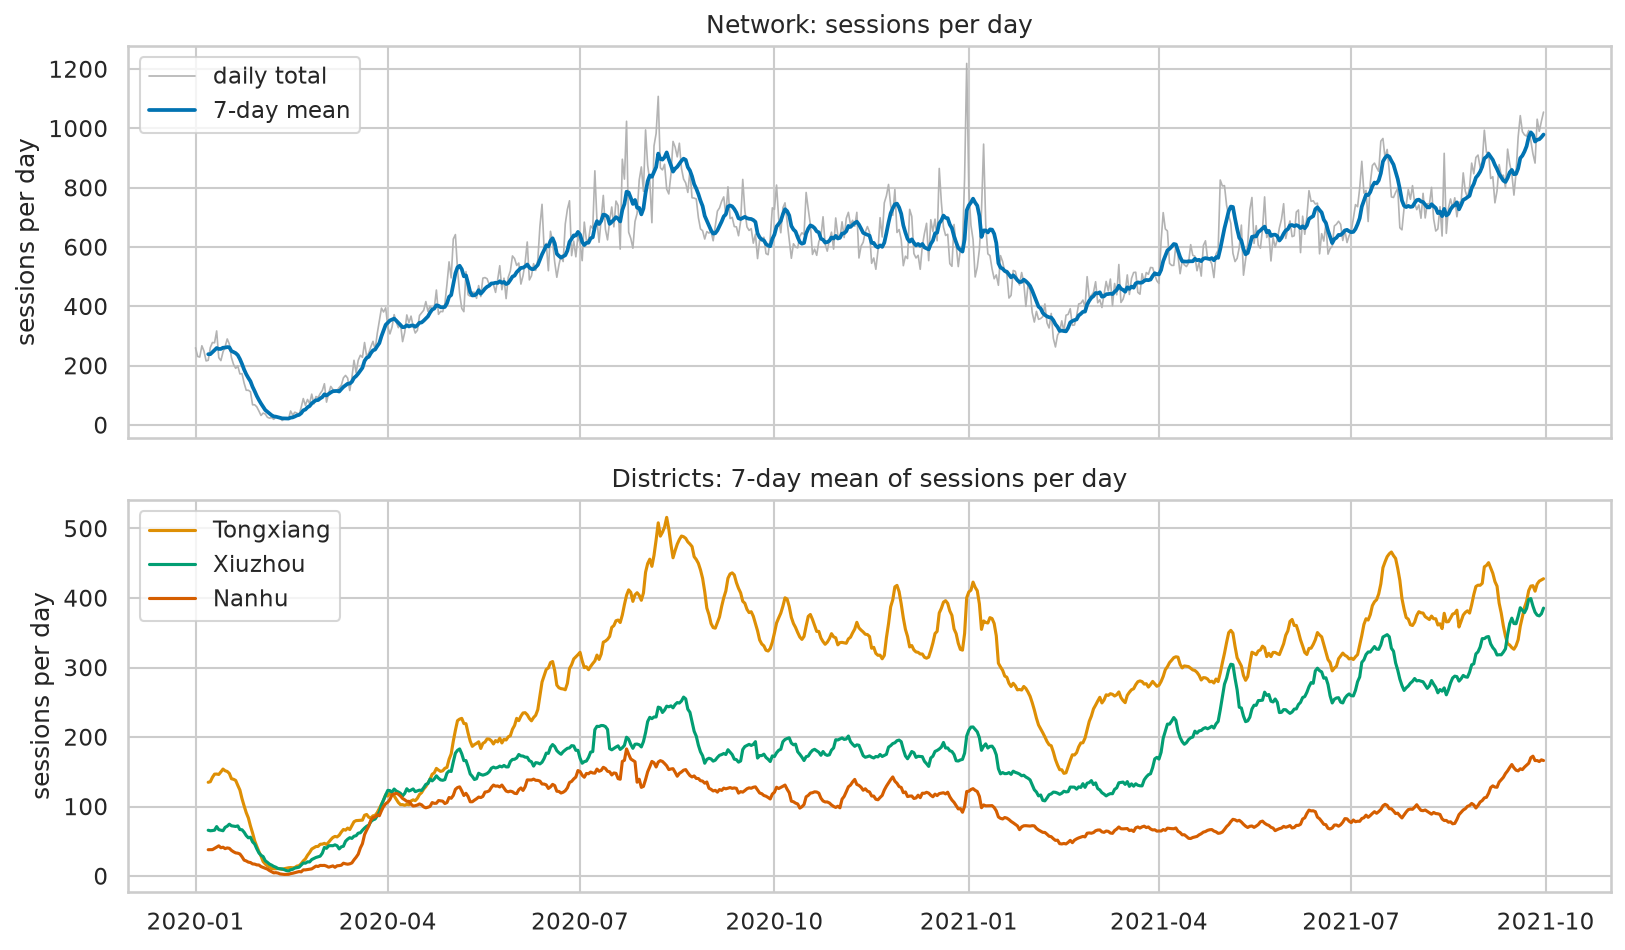
\includegraphics[width=\textwidth]{05_1_level_trend.png}
  \caption{Sessions per day for the network and 7-day means for the districts, 2020-01 to 2021-09}
  \label{fig:trend}
\end{figure}

Demand grows over the two years, but not smoothly (Figure~\ref{fig:trend}). The network went from 154 sessions per
day in the first quarter of 2020 to 737 in the third, fell to 464 in the first quarter of 2021, around the Spring
Festival, and reached 824 per day in the third quarter of 2021, its highest level. The districts do not move
together. Xiuzhou keeps growing (197 sessions per day in 2020-Q3, 320 in 2021-Q3), while Nanhu falls from 140 to 112
and stayed near 70 in the first half of 2021. A model trained on one period meets a different level in the next,
which is why the evaluation moves forward in time.

\section{Daily and weekly seasonality}\label{sec:season}

\begin{figure}[!htb]
  \centering
  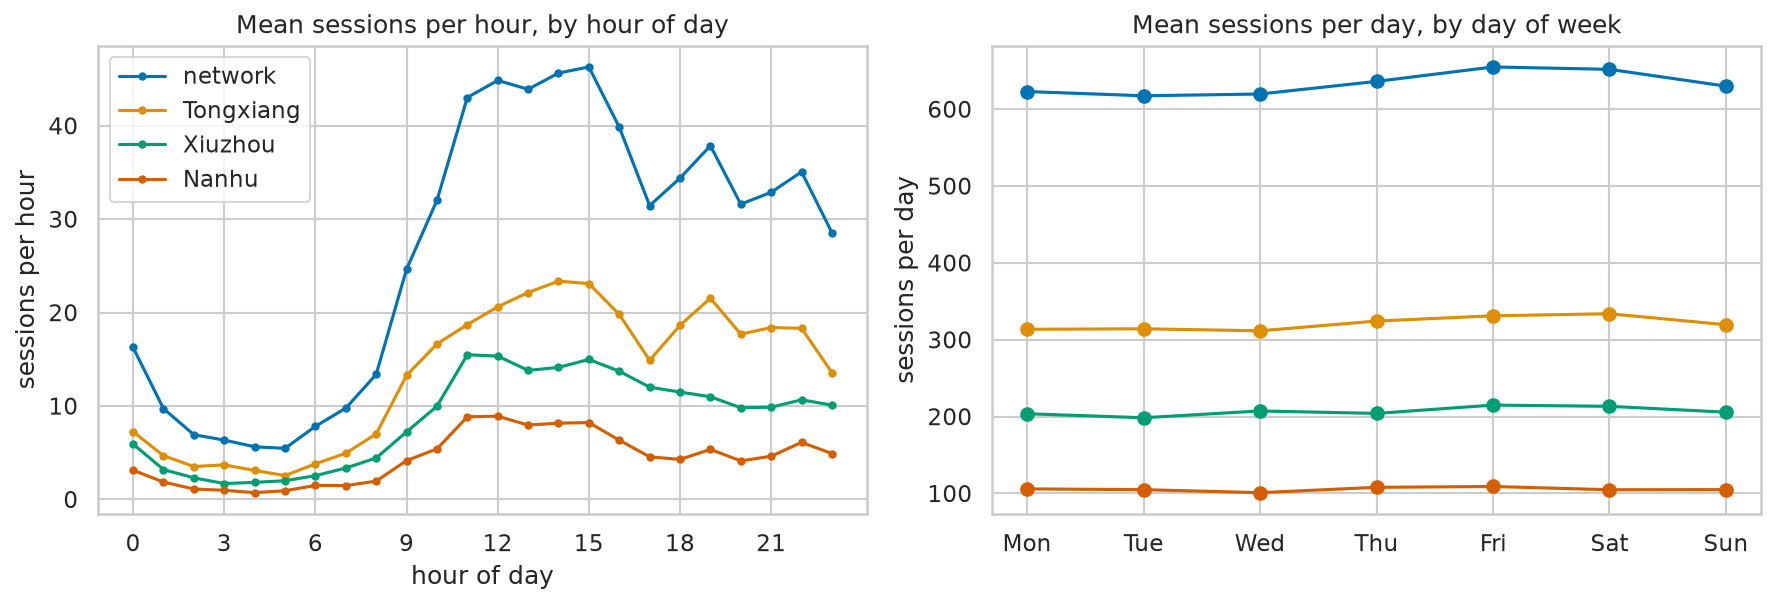
\includegraphics[width=\textwidth]{05_2_daily_weekly_profiles.png}
  \caption{Mean sessions per hour by hour of day and mean sessions per day by day of week, from 2020-04-01}
  \label{fig:profiles}
\end{figure}

The daily cycle is strong and the weekly one is weak (Figure~\ref{fig:profiles}). Network demand is lowest at 05:00
(5.5 sessions per hour) and highest at 15:00 (46.3), 8.5 times more. It climbs from 07:00 to a plateau between 11:00
and 15:00, falls at 16:00 and 17:00, and has smaller evening peaks at 19:00 and 22:00. The same shape appears on
every day of the week. Weekend days have only 1.7\% more sessions per day than weekdays at network level, and in
Nanhu slightly fewer.

\section{Autocorrelation and the seasonal period}\label{sec:acf}

The \ac{ACF} gives the correlation of a series with itself shifted by a number of hours. It is not covered in
class and was found through research~\cite{fpp3}. Figure~\ref{fig:acf} shows a peak at every multiple of 24 hours,
and the peak at 24 hours is higher than the one at 168 hours at every level (Table~\ref{tab:acf}). The seasonal naive
forecast, which repeats the value of one season earlier~\cite{fpp3}, agrees: repeating yesterday's hour gives a lower
error than repeating last week's at every level. The daily period is the stronger one, so \ac{MASE} is scaled with
$m = 24$.

\begin{figure}[!htb]
  \centering
  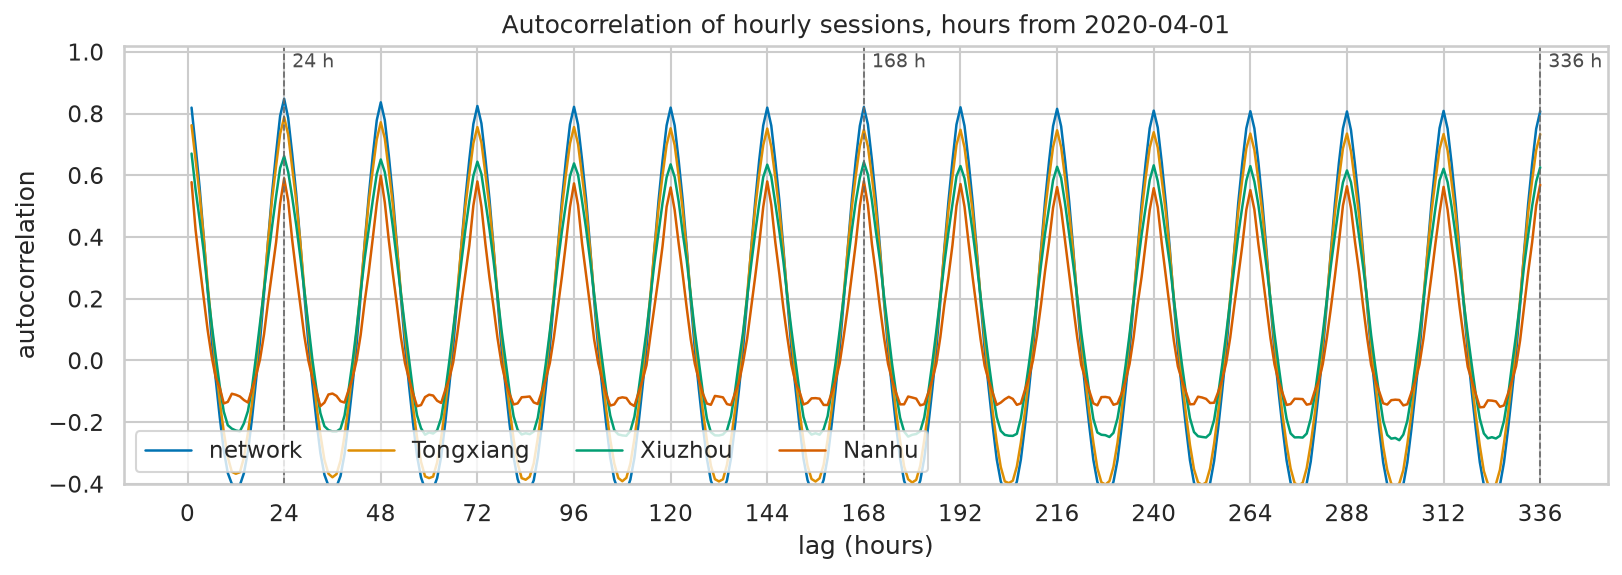
\includegraphics[width=\textwidth]{05_3_autocorrelation.png}
  \caption{Autocorrelation of hourly sessions at lags 1 to 336 hours, from 2020-04-01}
  \label{fig:acf}
\end{figure}

\begin{table}[!htb]
  \centering\small
  \caption{Autocorrelation at 24 and 168 hours and in-sample seasonal naive MAE (sessions per hour), from 2020-04-01}
  \label{tab:acf}
  \begin{tabular}{lrrrr}
    \toprule
    Level & ACF lag 24 & ACF lag 168 & MAE, $m=24$ & MAE, $m=168$ \\
    \midrule
    Network   & 0.848 & 0.821 & 7.12 & 7.63 \\
    Tongxiang & 0.788 & 0.748 & 4.48 & 4.83 \\
    Xiuzhou   & 0.662 & 0.642 & 4.19 & 4.27 \\
    Nanhu     & 0.590 & 0.581 & 2.53 & 2.55 \\
    \bottomrule
  \end{tabular}
\end{table}

\section{Holidays}\label{sec:holidays}

The holiday calendar comes from the State Council notices for 2020 and 2021~\cite{holidays2020,holidays2021}, which
are published months ahead. It marks 61 holiday days and 13 adjusted working days, the weekend days worked in
exchange for a longer holiday. Over the 548 days from 2020-04-01, holidays as a whole hardly change network demand
(0.99 times a normal weekday), but the average hides opposite effects: Tongxiang loses 5\% on holidays and Xiuzhou
gains 7\%. The Spring Festival is a real break. In its 2021 week the network averaged 327 sessions per day against
504 on the normal weekdays of the four weeks before, 35\% less (Figure~\ref{fig:holidays}). Adjusted working days
are not ordinary weekdays either: they have 9\% fewer sessions at network level and 16\% fewer in Tongxiang. Every
holiday is kept as legitimate variation, and models receive the two calendar flags instead of days being removed.

\begin{figure}[!htb]
  \centering
  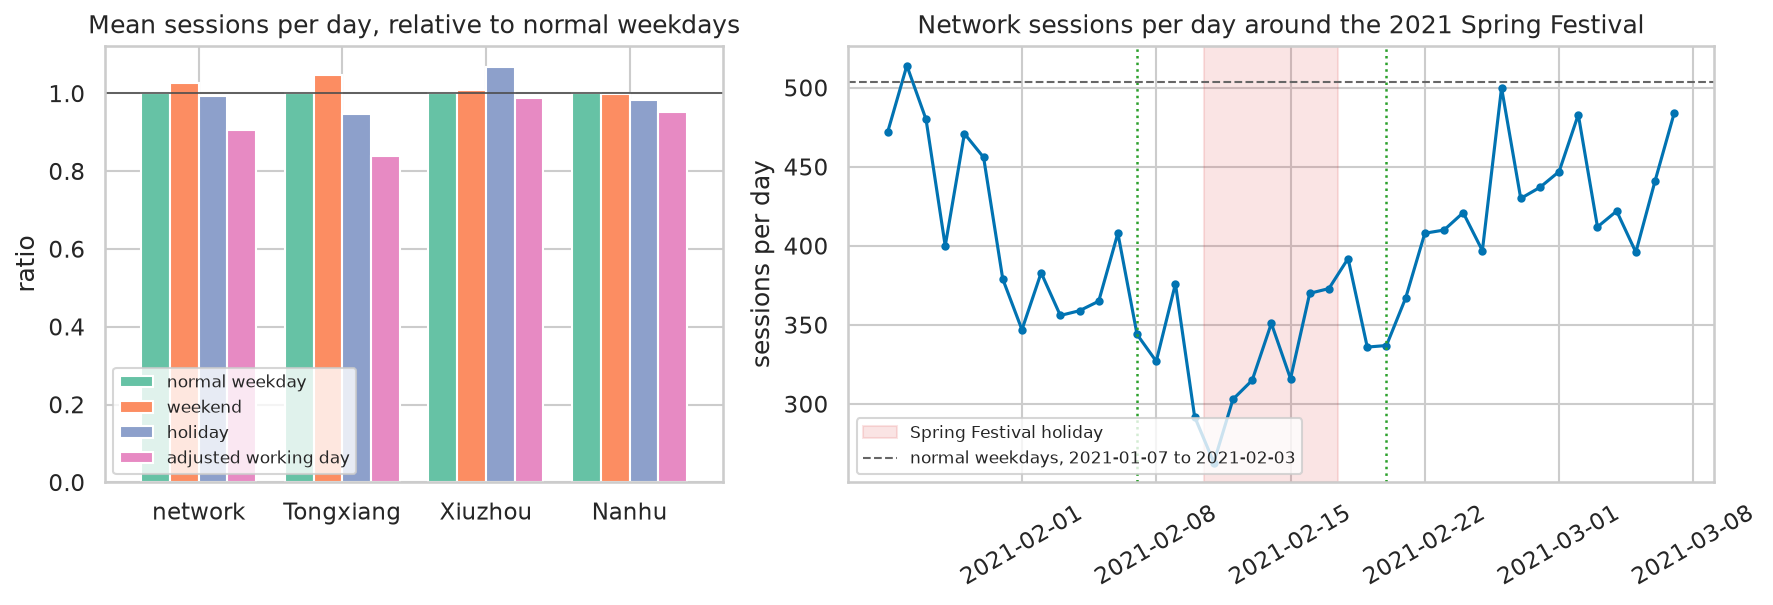
\includegraphics[width=\textwidth]{05_4_holidays.png}
  \caption{Mean sessions per day by day type relative to normal weekdays, and network demand around the 2021 Spring Festival}
  \label{fig:holidays}
\end{figure}

\section{The early-2020 restrictions and change over time}\label{sec:change}

February 2020 had 1,391 network sessions, against 6,217 in January and 6,392 in March. These are the first COVID-19
restrictions, and demand only came back in April (11,136 sessions) and May (15,033), as the left panel of
Figure~\ref{fig:change} shows. Those months describe an exceptional situation, so training rows start on 2020-04-01,
as in Project 1, and January to March 2020 serve only as lag history.

After April 2020 the level keeps changing but the daily shape does not. Between April--September 2020 and the same
months of 2021 network demand per day grew by 19.6\%, Xiuzhou by 60.4\% and Tongxiang by 17.0\%, while Nanhu fell by
29.5\%. The share of the day's sessions in each hour moved by at most 1.04 percentage points (right panel). A
forecaster therefore has to follow the level, while the shape of the day can be learnt from the whole training
window.

\begin{figure}[!htb]
  \centering
  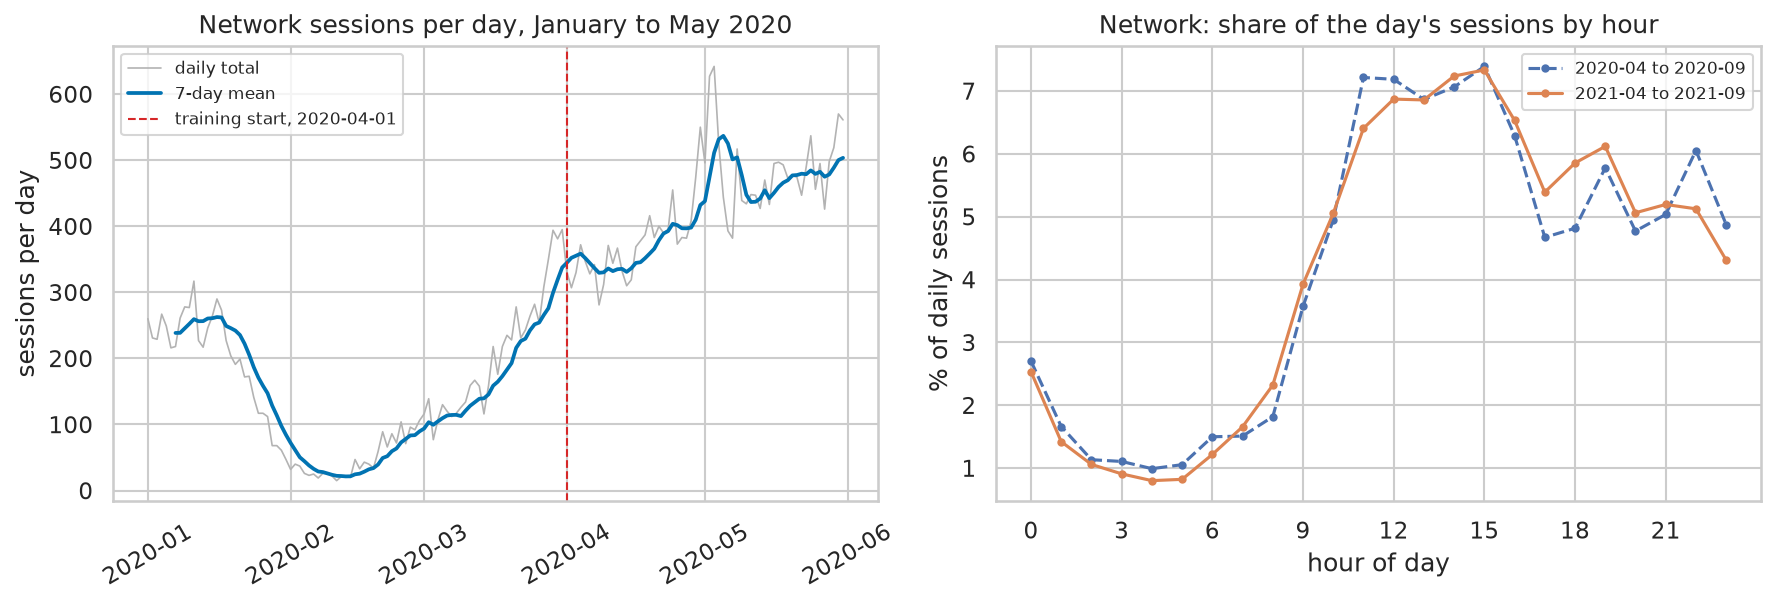
\includegraphics[width=\textwidth]{05_5_change_over_time.png}
  \caption{Network sessions per day from January to May 2020, and the hourly share of daily sessions in 2020 and 2021}
  \label{fig:change}
\end{figure}

\section{Districts}\label{sec:districts}

The districts differ mainly in size (Table~\ref{tab:districts}). Their hourly counts are overdispersed, with a
variance several times the mean, because the daily cycle moves the mean through the day. The smallest district has
the most empty hours. The shapes are close but not equal (Figure~\ref{fig:districts}): Xiuzhou and Nanhu peak before
noon, Tongxiang in the early afternoon with a stronger evening rise, and none has a weekly pattern larger than about
4\%. One shared model with the level as an input can learn these differences, while \ac{MASE} puts the districts on
the same scale.

\begin{table}[!htb]
  \centering\small
  \caption{District profiles, hours from 2020-04-01}
  \label{tab:districts}
  \begin{tabular}{lrrrrr}
    \toprule
    District & Share of sessions & Mean per hour & Variance / mean & Zero hours & Peak hour \\
    \midrule
    Tongxiang & 50.7\% & 13.4 & 6.9 & 2.1\% & 14:00 \\
    Xiuzhou   & 32.6\% &  8.6 & 6.0 & 6.5\% & 11:00 \\
    Nanhu     & 16.6\% &  4.4 & 3.9 & 15.0\% & 12:00 \\
    \bottomrule
  \end{tabular}
\end{table}

\begin{figure}[!htb]
  \centering
  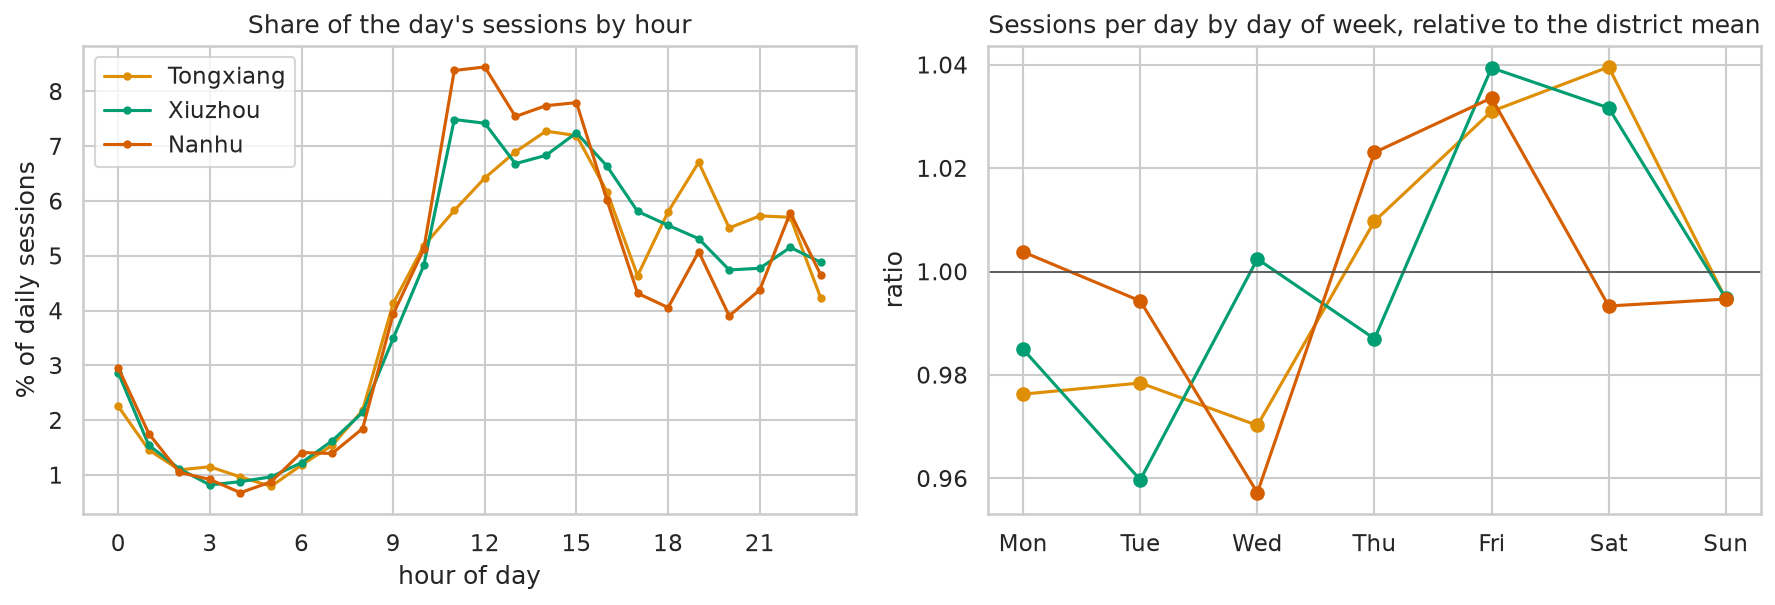
\includegraphics[width=\textwidth]{05_6_districts.png}
  \caption{Hourly share of daily sessions and day-of-week index by district, from 2020-04-01}
  \label{fig:districts}
\end{figure}

\section{Weather}\label{sec:weather}

Weather is recorded once per day and district, so only daily weather can be built from the file. Temperature is the
one variable that moves with demand, with a Spearman correlation of 0.62 with daily network sessions. Most of it is
seasonal, since temperature and demand both rise from spring to summer, so this does not show that warm days cause
charging. Humidity (0.04) and precipitation (0.01) show no relation, and rainy days have 0.98 times the sessions of
dry days. At 00:00 the weather of the coming day is not observed, so a model could only use a daily forecast, while
the file holds observed values. Weather therefore stays an exogenous candidate, to be tested in Task 2 under that
stated assumption.

%-------------------------------------------------------------- 4
\chapter{Forecasting Formulation}\label{ch:formulation}

\section{Issuance schedule}\label{sec:issuance}

A forecast is issued once a day at 00:00, using the data up to the hour that starts at 23:00 of the previous day. It
covers the 24 hours of that day: horizon 1 is 00:00 to 01:00 and horizon 24 is 23:00 to 24:00, so horizon $h$ is
always clock hour $h-1$. One forecast a day matches the daily planning of capacity and resources that the statement
describes. At midnight the same hour of the previous day is known for every horizon, and Section~\ref{sec:acf}
showed that this is the strongest single lag.

\section{Multi-step strategy}\label{sec:strategy}

There are three common ways to produce 24 values~\cite{bentaieb2012}; multi-step strategies are not covered in
class and were found through research. A recursive forecaster predicts one hour and feeds the prediction back
as an input for the next, so its errors pile up over the day. A direct forecaster with one model per horizon needs 24
models, each trained on a 24th of the data. The direct strategy with one shared model is used: each target hour of an
issuance is one row, all inputs of the row are known at 00:00, the hour of the day is one of the inputs, and no
forecast is fed back. The development period gives 52,608 such rows (548 issuances, 4 levels, 24 horizons), and none
is lost to gaps.

\section{Predictors and leakage}\label{sec:predictors}

Each candidate input is labelled as a historical observation, known future information or an exogenous variable
(Table~\ref{tab:catalogue}). A lag counted back from the target hour is known at 00:00 for every horizon only if it
is at least 24 hours: for horizon 24 (23:00), a lag of 23 hours would read 00:00 of the same day, which has not
happened yet. Windows counted back from the issuance, such as the previous day's total, end with the hour starting at
23:00 of the previous day and are known for every horizon. The function that builds the forecast rows works out the
latest hour each input reads and asserts, for every row, that it is before the issuance.

\begin{table}[!htb]
  \centering\small
  \caption{Predictor catalogue (Task 1 notebook, Section 6.3)}
  \label{tab:catalogue}
  \begin{tabularx}{\textwidth}{>{\raggedright\arraybackslash}p{4.6cm}>{\raggedright\arraybackslash}p{2.3cm}L}
    \toprule
    Input & Kind & Decision \\
    \midrule
    Same hour 24, 48 and 168 hours before; mean of the same hour over 7 days and over 4 weeks & Historical (from the target hour, lag $\geq 24$) & Included \\
    \addlinespace[2pt]
    Total of the previous day and of the previous 7 days & Historical (from the issuance) & Included \\
    \addlinespace[2pt]
    Hour of day, day of week, holiday, adjusted working day, month, level & Known future & Included \\
    \addlinespace[2pt]
    Daily temperature, humidity and precipitation as a forecast & Exogenous & Candidate for Task 2 \\
    \addlinespace[2pt]
    Observed weather of the target day; lags of 1 to 23 hours; any session after 00:00 & Exogenous / historical & Excluded: not known at issuance \\
    \addlinespace[2pt]
    Energy, costs, end cause, fault flags, user and post identifiers & Historical & Excluded: describe single sessions \\
    \bottomrule
  \end{tabularx}
\end{table}

\begin{figure}[!htb]
  \centering
  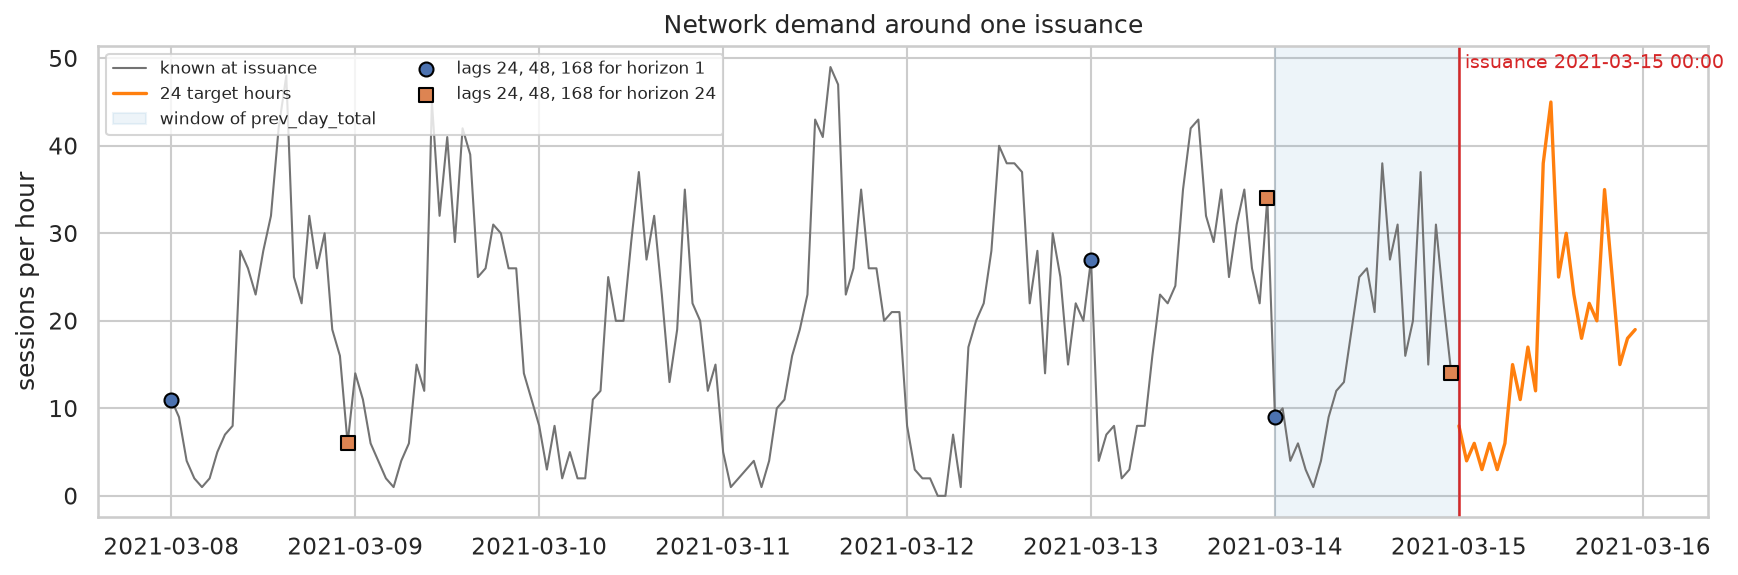
\includegraphics[width=\textwidth]{06_4_worked_issuance.png}
  \caption{One issuance, Monday 2021-03-15 at 00:00: known hours, target hours and the hours read by the lags}
  \label{fig:issuance}
\end{figure}

Figure~\ref{fig:issuance} shows one issuance. Everything left of the red line is known; the orange part is the 24
hours to forecast. For horizon 1 (00:00) the target was 8 sessions, against 9 at the same hour the day before and 11
a week before; for horizon 24 (23:00) it was 19, against 14 the day before. The previous day's total (413) and the
previous week's (3,216) are the same for all 24 rows, because they depend only on the issuance.

%-------------------------------------------------------------- 5
\chapter{Evaluation Protocol and Baselines}\label{ch:protocol}

\section{Folds}\label{sec:folds}

The four expanding-window folds of Project 1 are reused (Table~\ref{tab:folds}). Every fold trains from 2020-04-01 up
to the start of one validation quarter and validates on that quarter. Time order is kept, as the evaluation
deck~\cite{mindd04} requires for data that change over time, and each validation day is one issuance, so every model
is scored on the same 365 issuances. Project 1 purged a few sessions at each boundary; here demand is counted by
start hour, nothing crosses a boundary, and no gap is needed. In every fold the training sessions equal those of
Project 1 plus the sessions it purged, which confirms that both projects use the same data and periods.

\begin{table}[!htb]
  \centering\small
  \caption{Expanding-window folds (network sessions)}
  \label{tab:folds}
  \begin{tabular}{clrrr}
    \toprule
    Fold & Validation & Training days & Validation days & Validation sessions \\
    \midrule
    1 & 2020-Q4 & 183 & 92 & 60,364 \\
    2 & 2021-Q1 & 275 & 90 & 41,797 \\
    3 & 2021-Q2 & 365 & 91 & 57,542 \\
    4 & 2021-Q3 & 456 & 92 & 75,769 \\
    \bottomrule
  \end{tabular}
\end{table}

\section{Metrics and primary score}\label{sec:metrics}

\ac{MAE} and \ac{RMSE} are in sessions per hour~\cite{mindd04}; \ac{RMSE} weighs large misses more. \ac{MASE}, which
the statement asks for, divides the \ac{MAE} by the in-sample \ac{MAE} of the seasonal naive forecast on the
training hours of the same fold and level~\cite{hyndman2006}; it is not covered in class and was found through
research:
\[
  \text{MASE} = \frac{\frac{1}{n}\sum_{t} |y_t - \hat{y}_t|}{\frac{1}{T-m}\sum_{t=m+1}^{T} |y_t - y_{t-m}|},
  \qquad m = 24 .
\]
A value below 1 means the forecaster beats, on the validation quarter, what repeating yesterday's value achieved on
its training data. The scale is fitted on each fold's training hours only, so it is a learned operation and is
recorded in the ledger; every scale is positive, the smallest being 2.54 sessions per hour (Nanhu, fourth fold).

Choosing between forecasters requires one number. The primary score averages \ac{MASE} over the 24 horizons, then
over the four levels with equal weight, then over the four folds, and the four fold values are always reported
beside it. Because \ac{MASE} has no unit, Nanhu counts as much as the network. \ac{MAE} and \ac{RMSE} per level
remain secondary scores, since they say how many sessions a forecast misses. Results can also be broken down by
horizon, by month and by day type.

\section{Baselines}\label{sec:baselines}

The baselines need no fitting and are all legal at 00:00. The daily seasonal naive repeats the same hour one day
earlier, the weekly seasonal naive the same hour one week earlier, and the four-week mean averages the same hour and
weekday over the four previous weeks. Table~\ref{tab:baselines} gives their scores.

\begin{table}[!htb]
  \centering\small
  \caption{Baseline scores on the development folds: primary MASE per fold and overall, mean MASE per level, and MAE (sessions per hour)}
  \label{tab:baselines}
  \setlength{\tabcolsep}{3.6pt}
  \begin{tabular}{lrrrrrrrrrr}
    \toprule
    & \multicolumn{5}{c}{Primary MASE} & \multicolumn{4}{c}{MASE per level} & MAE \\
    \cmidrule(lr){2-6}\cmidrule(lr){7-10}\cmidrule(lr){11-11}
    Baseline & F1 & F2 & F3 & F4 & All & Net. & Tong. & Xiu. & Nan. & Net. \\
    \midrule
    Daily naive   & 1.007 & 0.827 & 0.999 & 1.167 & 1.000 & 1.022 & 1.033 & 1.130 & 0.814 & 7.14 \\
    Weekly naive  & 1.066 & 0.860 & 1.048 & 1.216 & 1.047 & 1.096 & 1.111 & 1.158 & 0.824 & 7.65 \\
    Four-week mean & 0.854 & 0.782 & 0.829 & 1.012 & \textbf{0.869} & 0.916 & 0.926 & 0.940 & 0.695 & 6.40 \\
    \bottomrule
  \end{tabular}
\end{table}

The four-week mean is the best in every fold and at every level: averaging four weeks removes much of the
hour-to-hour noise that a single copied value carries. The weekly naive is the worst, as the weak weekly pattern
suggested. Figure~\ref{fig:baselines} shows how the errors depend on the hour. All three baselines have a \ac{MASE}
around 0.4 in the night hours, when few sessions start; for the network and the two larger districts they exceed 1
for most hours between 10:00 and 20:00, when demand is high and changes most from day to day, while Nanhu stays closer
to 1. The fourth fold is the hardest, because demand grew fast in the third quarter of 2021, and holidays are the
hardest day type (0.985 for the four-week mean against 0.865 on normal weekdays). In sessions, the four-week mean
misses the network by 6.4 sessions per hour on average (\ac{RMSE} 8.2) and Nanhu by 1.9. It is the reference
baseline: a model is useful only if it beats 0.869 on the same folds.

\begin{figure}[!htb]
  \centering
  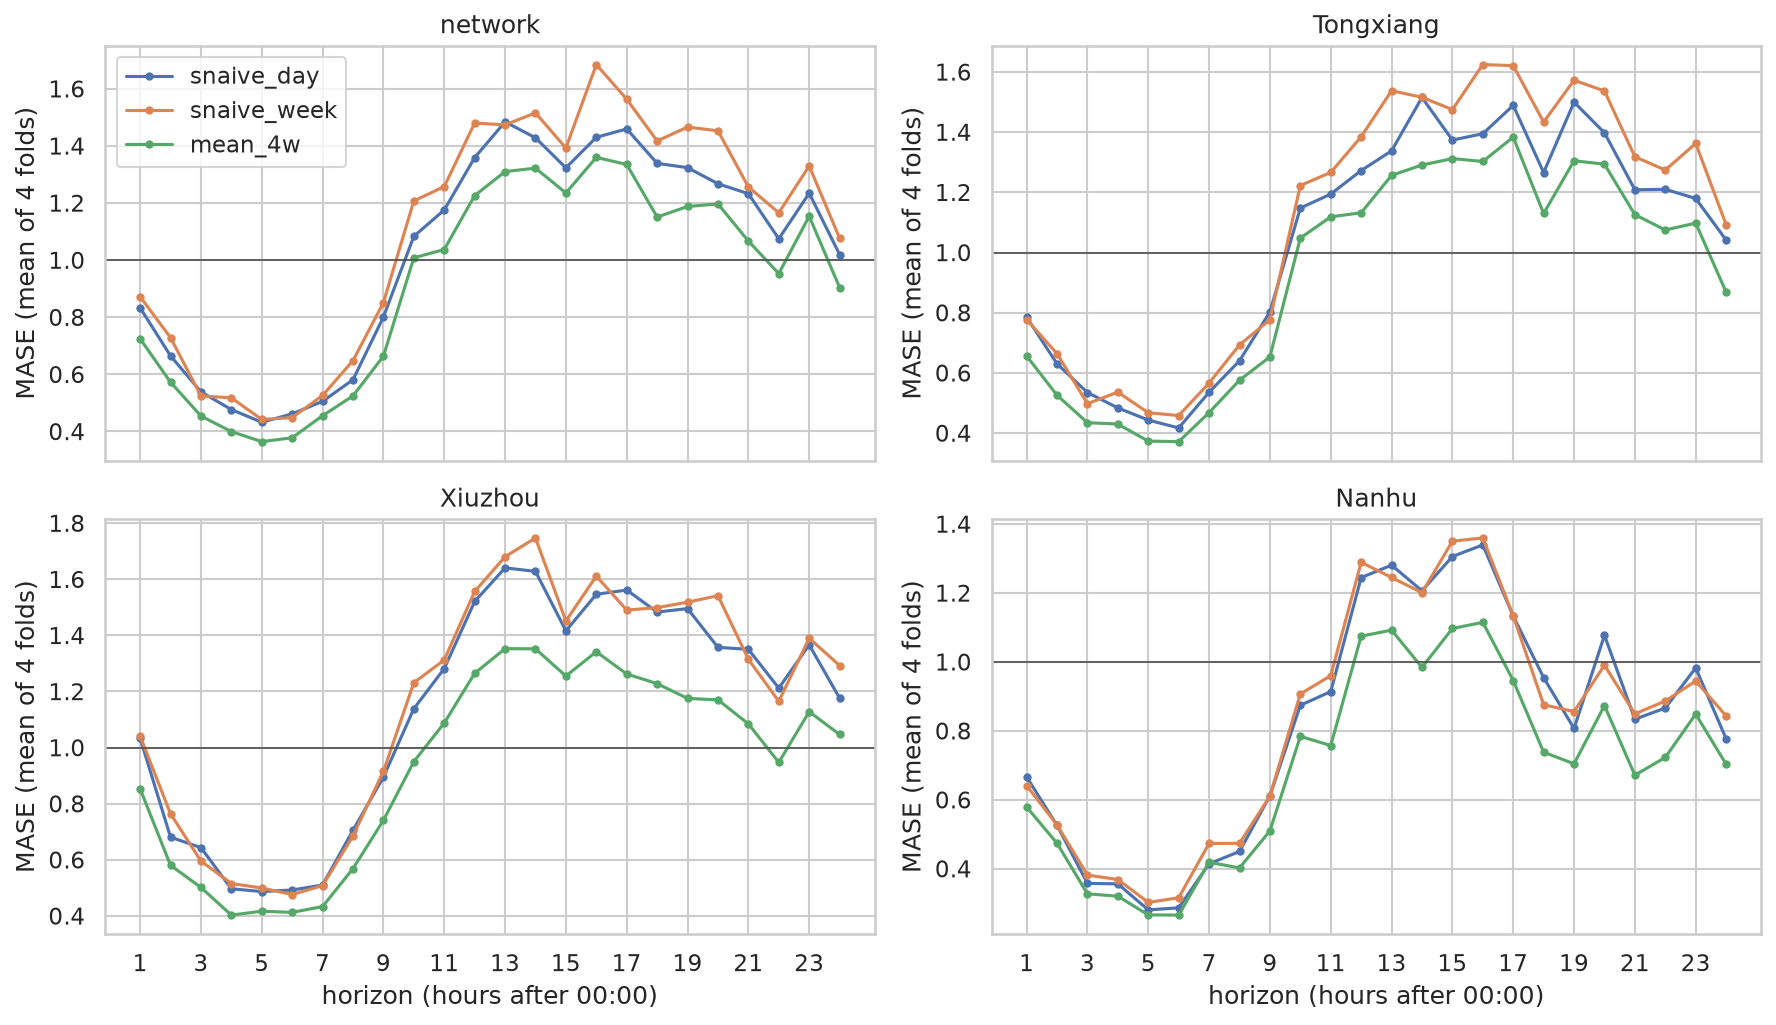
\includegraphics[width=\textwidth]{07_5_baselines_by_horizon.png}
  \caption{MASE by horizon for the three baselines, mean of the four folds}
  \label{fig:baselines}
\end{figure}

\section{Saved protocol}\label{sec:saved}

The protocol file \texttt{task1\_protocol.json} holds the problem definition, the data fingerprint, the periods, the
folds, the predictors with the leakage rule, the metrics, the breakdowns and the baselines. With the hourly series it
is enough to rebuild the folds and recompute any baseline score; this was checked in a fresh session for one score
(fold 2, Xiuzhou, horizon 9). Two runs of the notebook give identical files apart from the run date and times, and a
full run needs less than ten seconds of computation.

%-------------------------------------------------------------- 6
\chapter{Statistical Forecasting Models}\label{ch:stat}

Task 2 asks which statistical time-series methods suit the problem and how they compare with the
baselines~\cite{brief}. The models were chosen from what Task 1 found in the series: a strong daily cycle, a weak
weekly one, a level that changes from quarter to quarter, and holidays that break the pattern. \ac{ETS}, \ac{ARIMA},
\ac{SARIMAX} and \ac{MSTL} are not covered in class and were found through research~\cite{fpp3,bandara2021}.

\section{Protocol}\label{sec:stat-protocol}

The protocol of Task 1 is used unchanged: the same series, folds, test period, metrics, primary score and baselines.
The statement asks for that protocol to be ``finalized before proceeding to model development''~\cite{brief}, and the
baseline scores per fold were already known, so a new split at this point would be chosen after seeing results. The
shortest training window, 26 weeks in the first fold, holds enough daily and weekly cycles for these models. Before
any model is scored, the Task 2 scoring function recomputes the baseline primary scores of Task 1 (0.869, 1.000 and
1.047), and the SHA-256 of every Task 1 file is the same at the end of the run as at the start.

One part of the protocol needs a narrower scope. The direct strategy with one shared model
(Section~\ref{sec:strategy}) is a layout of rows for feature-based models. A statistical model produces the 24 values
of a day from its own equations, starting from its state at 00:00. That state may use every hour up to the one
starting at 23:00 of the previous day, the information set of Section~\ref{sec:issuance}. The direct
strategy stays for the feature-based models of the later tasks.

\section{Models and the two cycles}\label{sec:models}

Five variants of four families were fitted to each of the four series (Table~\ref{tab:models}). The \ac{ETS} model
has an additive season of 24 hours~\cite[Chapter 8]{fpp3}. \ac{SARIMA} differences the series at lag 24 and models
what remains with short and seasonal terms~\cite[Chapter 9]{fpp3}. \ac{SARIMAX} adds regression inputs to the same
structure, with \ac{SARIMA} errors~\cite[Chapter 10]{fpp3}. Its calendar inputs are published in advance, and the
temperature is the recorded value of the day, read as the forecast available at 00:00. \ac{MSTL} splits the training
hours into a trend, a daily and a weekly seasonal part~\cite{bandara2021}; the two seasonal parts of the last
training week are repeated forward, and an \ac{ARIMA} with a constant forecasts the rest.

\begin{table}[!htb]
  \centering\small
  \caption{The five model variants and how they treat the daily and weekly cycles}
  \label{tab:models}
  \begin{tabularx}{\textwidth}{>{\raggedright\arraybackslash}p{2.7cm}>{\raggedright\arraybackslash}p{3.3cm}>{\raggedright\arraybackslash}p{3.0cm}L}
    \toprule
    Model & Daily cycle & Weekly cycle & Inputs \\
    \midrule
    \col{ets} & Season of 24 hours & Only through the state & None \\
    \col{sarima} & Seasonal difference and MA term at 24 hours & Only through the state & None \\
    \col{sarimax_cal} & As \col{sarima} & Day-of-week inputs & Six day-of-week dummies, holiday and adjusted-working-day flags \\
    \col{sarimax_weather} & As \col{sarima} & Day-of-week inputs & As \col{sarimax_cal}, plus the temperature of the day \\
    \col{mstl_arima} & Seasonal part of 24 hours & Seasonal part of 168 hours & None \\
    \bottomrule
  \end{tabularx}
\end{table}

Only \ac{MSTL} represents both cycles explicitly. \ac{ETS} and \ac{SARIMA} carry the weekly cycle only through what
the last days left in their state, a limited loss given how weak the weekly pattern is (Section~\ref{sec:season}).
None of the models has a yearly cycle.

\section{Transformation and daily forecasting}\label{sec:transform}

Hourly counts are small and their spread grows with their level. On the training hours of the first fold, the
largest standard deviation of a clock hour is 4.5 to 5.4 times the smallest on the count scale, and 1.5 to 2.0 times
on the log scale. Every model is therefore fitted to $\log(1 + \text{count})$, the log transform of the data
preparation deck~\cite{mindd03}, which keeps the zeros. A forecast comes back as $\max(e^{x} - 1, 0)$. The clip acts
only when $x < 0$, so it removes less than one session each time. It acted at most 4 times in 35,040 forecasts for
\ac{ETS}, \ac{SARIMA} and \ac{SARIMAX}, always in Nanhu, and 392 times for \ac{MSTL} + \ac{ARIMA}. Taken back from
the log scale, a forecast is a median-type value, slightly below the mean of the count, which weighs more on
\ac{RMSE} than on \ac{MAE}.

Coefficients are estimated once per fold and level on the training hours. Within the validation quarter the model is
run over the observed hours with these fixed coefficients, and each 00:00 issuance takes a 24-hour forecast that uses
only the hours before it. Re-estimating every day would mean about 90 fits per fold and level. To check that no
later hour reaches a forecast, the network counts of the second fold from 2021-02-01 00:00 on were multiplied by 10
and the forecast issued at that midnight was recomputed: it did not change for any of the five models.

\section{Structure selection}\label{sec:selection}

Each structure was chosen once per level on the training hours of the first fold (2020-04-01 to 2020-09-30) and
kept for the four folds; only the coefficients change from fold to fold. For \ac{SARIMA} the lag-24 difference
follows from the daily cycle. The \ac{ADF} test~\cite{dickeyfuller1979} and the \ac{KPSS} test~\cite{kpss1992}, not
covered in class and found through research, agree after that difference at every level (\ac{ADF} p-value 0.000,
\ac{KPSS} p-value 0.100), so no further difference is taken. The \ac{ACF} of the differenced series has a small spike
at lag 1 (0.076 to 0.115) and a large negative one at lag 24 ($-0.508$ to $-0.479$), which points to short
\ac{ARIMA} terms and a seasonal MA term. A short list of candidates per family was compared by \ac{AIC}
(Table~\ref{tab:structures}). \ac{AIC} is compared only within a family, because the families are fitted to
different versions of the series.

\begin{table}[!htb]
  \centering\small
  \caption{Candidates compared by AIC on the first fold and the structure chosen (the same at every level)}
  \label{tab:structures}
  \begin{tabularx}{\textwidth}{>{\raggedright\arraybackslash}p{2.5cm}L>{\raggedright\arraybackslash}p{3.4cm}r}
    \toprule
    Model & Candidates & Chosen & AIC gap \\
    \midrule
    \ac{ETS} & no trend; damped trend & no trend & 3.2 to 6.0 \\
    \ac{SARIMA} & $(p,0,q)(P,1,Q)_{24}$, $p \in \{1,2\}$, $q \in \{0,1\}$, $(P,Q) \in \{(0,1),(1,1)\}$ & $(2,0,1)(0,1,1)_{24}$ & 0.2 to 1.9 \\
    \ac{MSTL} + \ac{ARIMA} & $\text{ARIMA}(p,0,q)$ with a constant, $p \in \{1,2\}$, $q \in \{0,1\}$ & $\text{ARIMA}(2,0,1)$ with a constant & 9.8 to 35.8 \\
    \ac{SARIMAX} & the \ac{SARIMA} structure of the level & $(2,0,1)(0,1,1)_{24}$ & -- \\
    \bottomrule
  \end{tabularx}
\end{table}

The same structure won at every level. The \ac{SARIMA} gaps are small: a seasonal AR term adds 0.2 to 1.9 \ac{AIC}
points, so the seasonal MA term already carries the daily cycle. The damped trend of \ac{ETS} adds two coefficients
that barely improve the likelihood. The two \ac{SARIMAX} variants keep the \ac{SARIMA} structure of their level, so
their comparison with \ac{SARIMA} shows the effect of the inputs alone.

\section{Residual diagnostics}\label{sec:diagnostics}

Residuals are taken on the log scale over the training hours of each fold, without the first 192 hours. The
Ljung-Box test~\cite{ljungbox1978}, not covered in class and found through research, asks whether autocorrelation
remains up to 24 and 168 hours. With 4,200 to 10,752 hours it rejects white noise for almost any real series, so the
size of the remaining autocorrelation matters more than the p-value~\cite[Section 5.4]{fpp3}
(Table~\ref{tab:residuals}).

\begin{table}[!htb]
  \centering\small
  \caption{Residual autocorrelation at 24 and 168 hours (range over levels of the mean over folds), largest
  Ljung-Box p-value over the 16 cells, and mean residual on holidays (log scale)}
  \label{tab:residuals}
  \setlength{\tabcolsep}{4pt}
  \begin{tabular}{lrrrr}
    \toprule
    Model & ACF lag 24 & ACF lag 168 & Largest $p$ & Holiday mean \\
    \midrule
    \col{ets}             & $-0.007$ to $0.021$ & $0.003$ to $0.033$ & 0.001 & $-0.002$ \\
    \col{sarima}          & $-0.010$ to $0.020$ & $0.003$ to $0.028$ & 0.565 & $0.021$ \\
    \col{sarimax_cal}     & $-0.009$ to $0.019$ & $0.001$ to $0.027$ & 0.496 & $-0.011$ \\
    \col{sarimax_weather} & $-0.008$ to $0.020$ & $0.002$ to $0.027$ & 0.389 & $-0.012$ \\
    \col{mstl_arima}      & $-0.265$ to $-0.245$ & $-0.164$ to $-0.148$ & 0.000 & $-0.009$ \\
    \bottomrule
  \end{tabular}
\end{table}

For \ac{ETS}, \ac{SARIMA} and \ac{SARIMAX} the remaining autocorrelation is at most 0.033 in absolute value, and a
few \ac{SARIMA} and \ac{SARIMAX} cells even pass the test (Figure~\ref{fig:residuals}). \ac{MSTL} + \ac{ARIMA} leaves
about $-0.25$ at lag 24 and $-0.15$ at lag 168 at every level. The seasonal parts seem to take up some of the noise
of single days and weeks, and subtracting them leaves an echo of opposite sign. The mean residuals are small, about
2\% of the count at most. The holiday flags of \ac{SARIMAX} turn the $+0.021$ of \ac{SARIMA} on holidays into
$-0.011$, and night and day residuals differ by less than 0.002 for every model. The distributions are close to
normal, with a slightly longer left tail from hours with far fewer sessions than expected.

\begin{figure}[!htb]
  \centering
  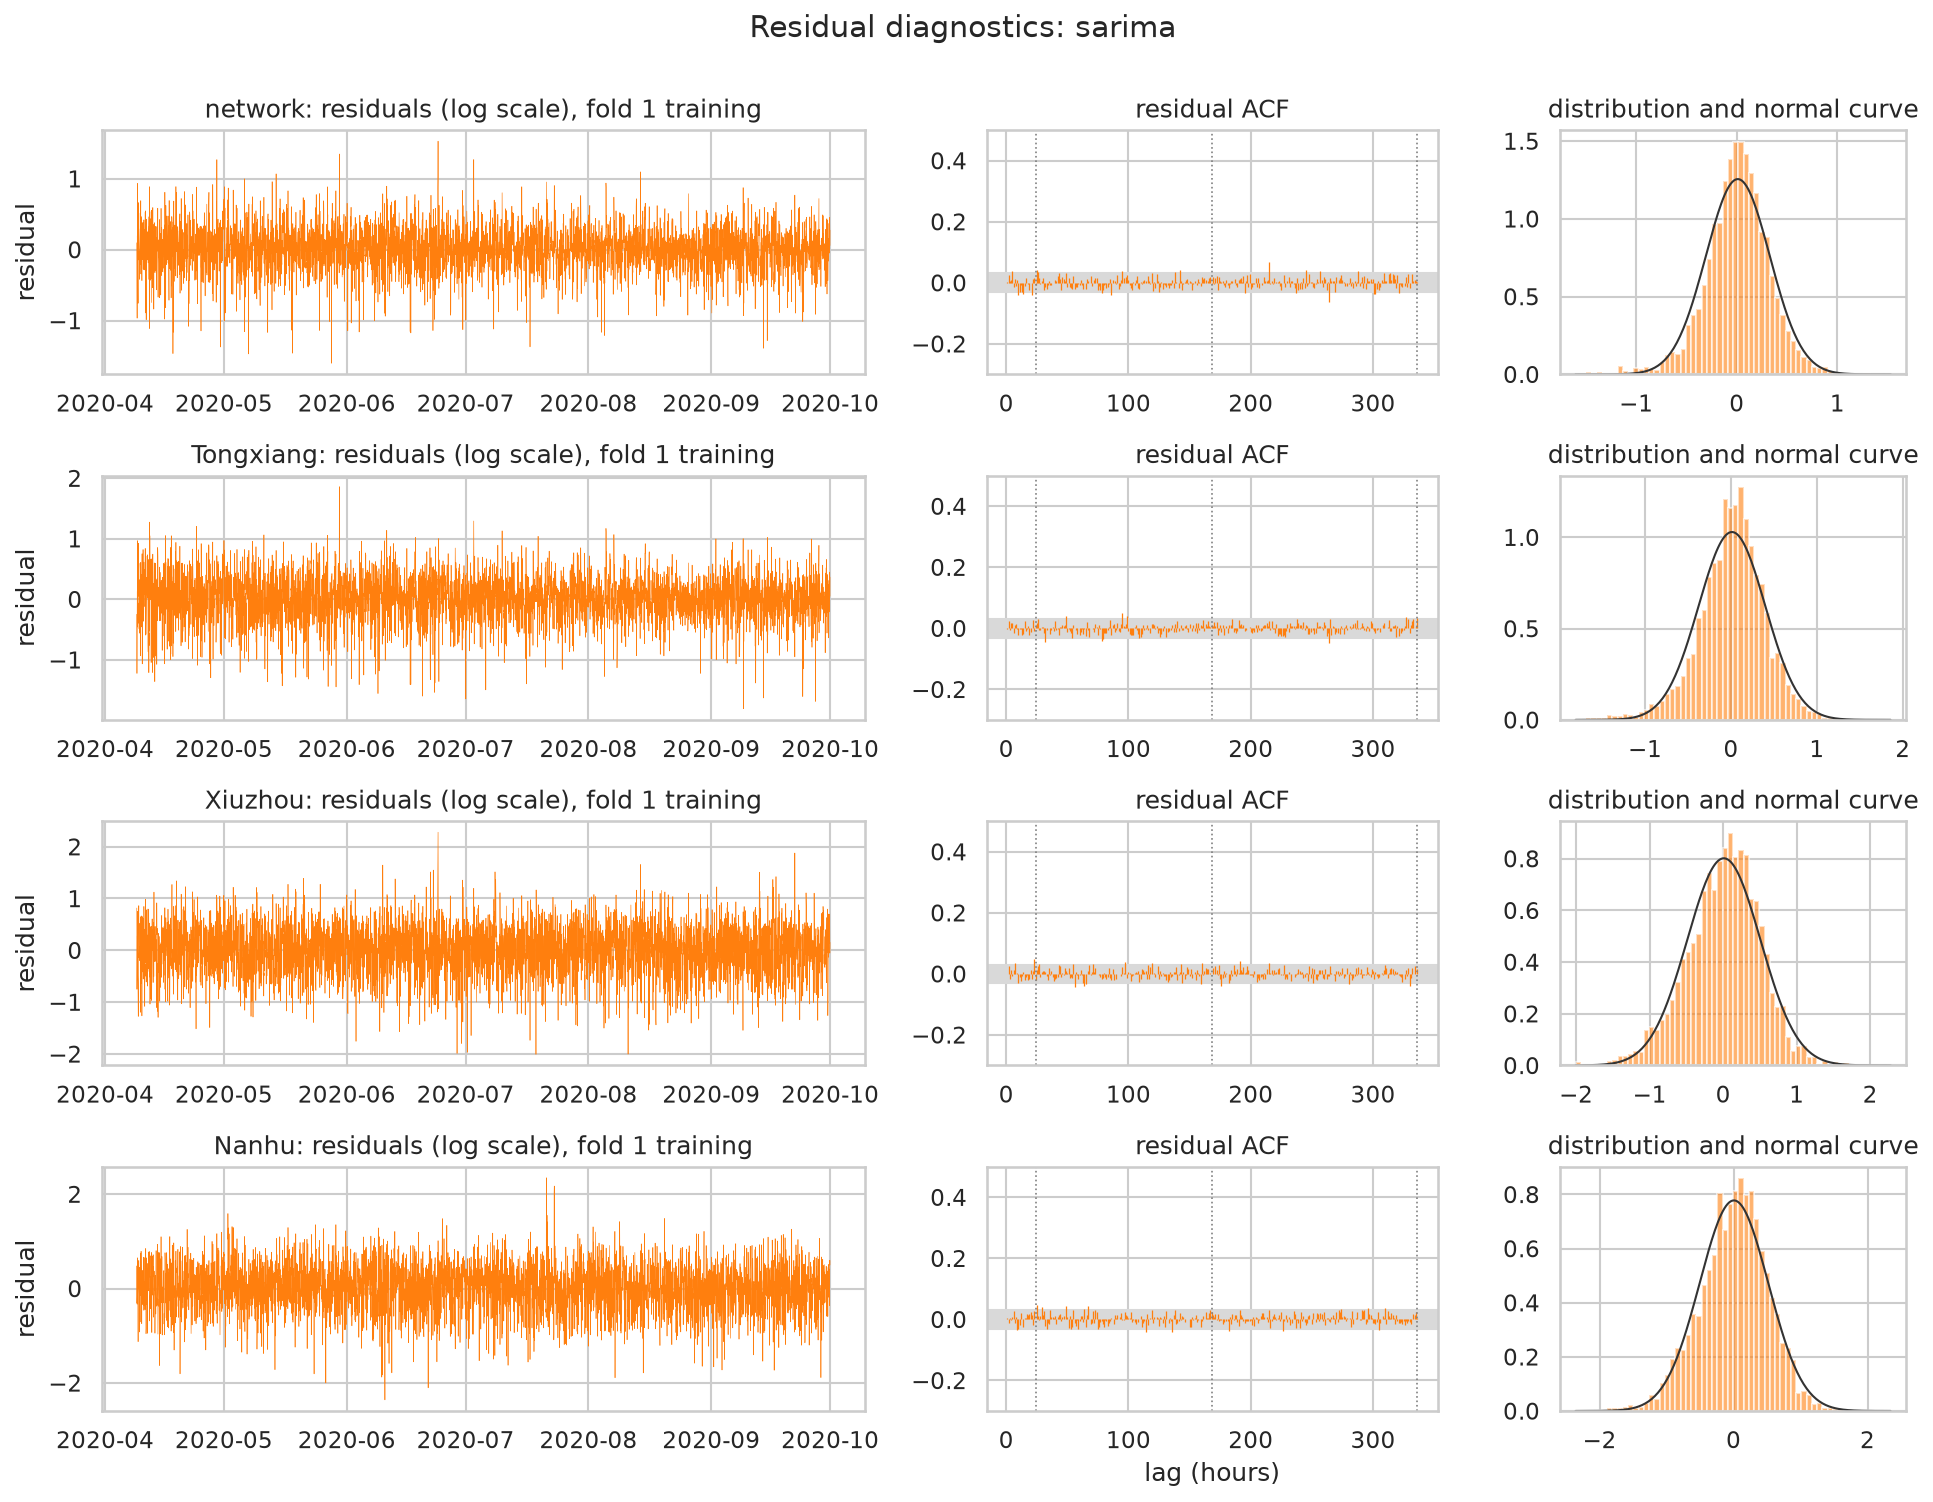
\includegraphics[width=\textwidth]{07_sarima_residuals.png}
  \caption{Residuals of \texttt{sarima} on the training hours of the first fold: over time, autocorrelation up to 336
  hours, and distribution with a normal curve}
  \label{fig:residuals}
\end{figure}

\section{Comparison with the baselines}\label{sec:comparison}

Four of the five models beat the four-week mean in every one of the 16 combinations of level and fold
(Table~\ref{tab:comparison} and Figure~\ref{fig:primary}). \ac{SARIMAX} with calendar inputs has the lowest primary
\ac{MASE} (0.7536), followed by \ac{SARIMA} (0.7544) and \ac{ETS} (0.7557), all about 13\% below 0.869. The three
differ by less than 0.002, much less than the spread between folds, so their order carries little weight: three
different families reach the same level. In sessions, they miss network demand by 5.4 to 5.5 per hour, against 6.4
for the four-week mean, and Nanhu by 1.7 against 1.9. \ac{MSTL} + \ac{ARIMA}, at 0.910, does worse than the reference
overall and in 14 of the 16 cells, because its seasonal parts repeat the last training week over a whole quarter.

\begin{table}[!htb]
  \centering\small
  \caption{Primary MASE per fold and overall, cells (of 16) below the four-week mean, and network MAE and RMSE
  (sessions per hour)}
  \label{tab:comparison}
  \setlength{\tabcolsep}{4pt}
  \begin{tabular}{lrrrrrrrr}
    \toprule
    & \multicolumn{5}{c}{Primary MASE} & & \multicolumn{2}{c}{Network} \\
    \cmidrule(lr){2-6}\cmidrule(lr){8-9}
    Method & F1 & F2 & F3 & F4 & All & Cells & MAE & RMSE \\
    \midrule
    \col{sarimax_cal}     & 0.768 & 0.619 & 0.743 & 0.884 & \textbf{0.754} & 16 & 5.42 & 7.06 \\
    \col{sarima}          & 0.768 & 0.613 & 0.754 & 0.882 & 0.754 & 16 & 5.43 & 7.06 \\
    \col{ets}             & 0.772 & 0.619 & 0.752 & 0.879 & 0.756 & 16 & 5.47 & 7.12 \\
    \col{sarimax_weather} & 0.798 & 0.619 & 0.745 & 0.884 & 0.762 & 16 & 5.50 & 7.20 \\
    \col{mstl_arima}      & 0.896 & 0.743 & 0.893 & 1.107 & 0.910 & 2  & 6.45 & 8.32 \\
    \midrule
    Four-week mean        & 0.854 & 0.782 & 0.829 & 1.012 & 0.869 & -- & 6.40 & 8.22 \\
    Daily naive           & 1.007 & 0.827 & 0.999 & 1.167 & 1.000 & 2  & 7.14 & 9.20 \\
    Weekly naive          & 1.066 & 0.860 & 1.048 & 1.216 & 1.047 & 0  & 7.65 & 9.85 \\
    \bottomrule
  \end{tabular}
\end{table}

\begin{figure}[!htb]
  \centering
  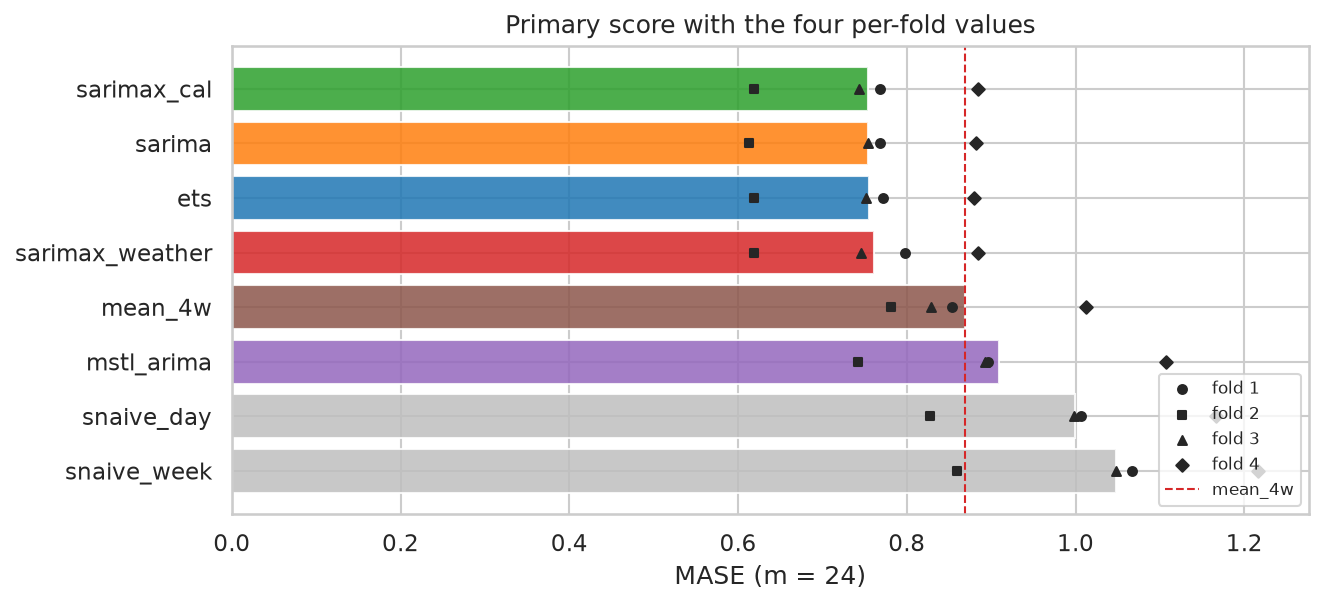
\includegraphics[width=0.85\textwidth]{08_1_primary_mase.png}
  \caption{Primary MASE of every method with its four per-fold values; the dashed line is the four-week mean}
  \label{fig:primary}
\end{figure}

\section{Stability over time, horizons and levels}\label{sec:stability}

The gain holds in every fold: per fold the four models score 0.613 to 0.884, against 0.782 to 1.012 for the
four-week mean. The fourth fold, with the fast growth of 2021-Q3, is the hardest for every method, and September
2021 is the worst month (0.971 to 0.976, against 1.112, averaged over levels). By horizon, the error follows the
daily cycle of demand more than the distance from midnight (Figure~\ref{fig:stat-horizon}). Night hours are easy for
every method, and the midday and afternoon hours stay near or above 1 at the three larger levels. The models gain
the most where the baseline errs the most, for example 1.03 to 1.05 against 1.17 at horizon 12 (11:00), averaged
over levels and folds.

\begin{figure}[!htb]
  \centering
  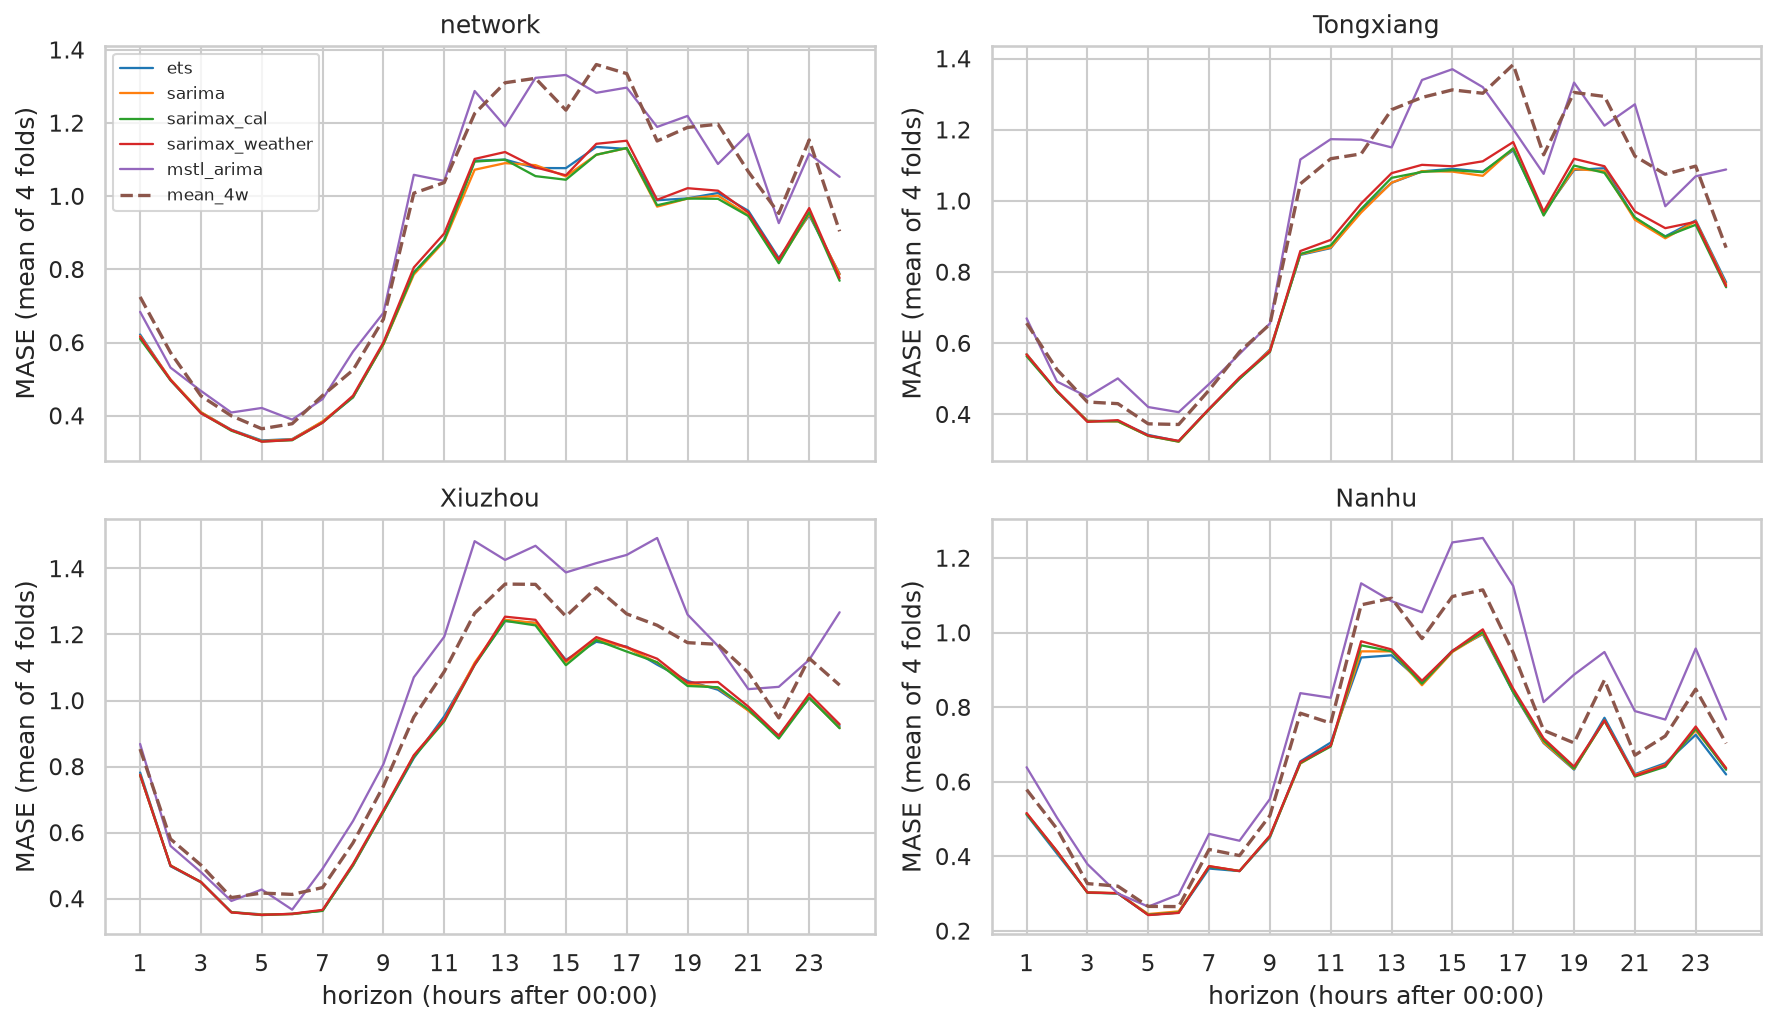
\includegraphics[width=\textwidth]{09_1_mase_by_horizon.png}
  \caption{MASE by horizon for the five models and the four-week mean (dashed), mean of the four folds}
  \label{fig:stat-horizon}
\end{figure}

The second fold, which contains the 2021 Spring Festival, is the easiest for the models (0.613 to 0.619) and the one
where they gain the most over the four-week mean (0.782). In February 2021 their \ac{MASE}, averaged over levels, is
0.552 to 0.557 against 0.768 (Figure~\ref{fig:stat-month}). A model that updates its state every day follows the
holiday drop within a day or two, while a four-week average carries the earlier level into the holiday weeks.
Holidays remain the hardest day type for every model (0.856 to 0.860, against 0.744 to 0.755 on normal weekdays), and
the holiday flag of \ac{SARIMAX} does not lower that error. Xiuzhou is the hardest level and Nanhu the easiest, as for
the baselines (Table~\ref{tab:stat-levels}).

\begin{figure}[!htb]
  \centering
  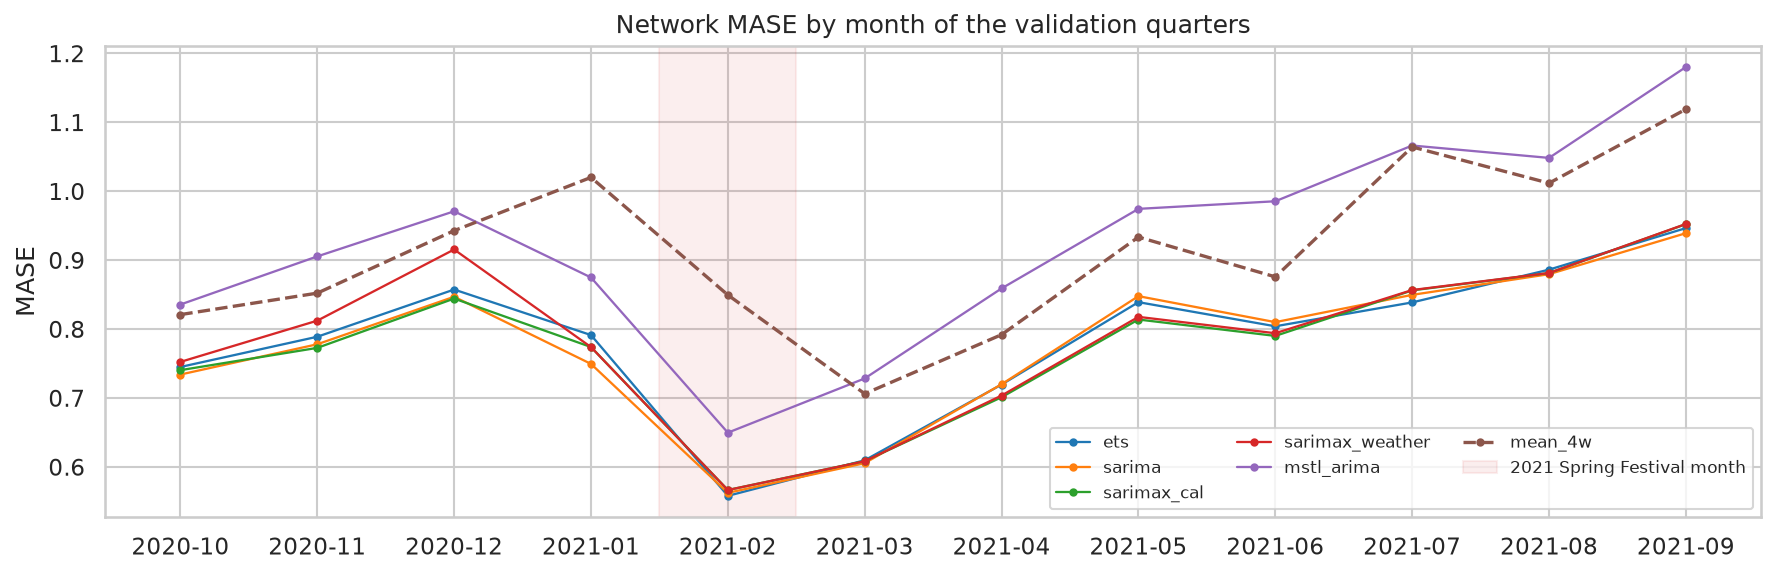
\includegraphics[width=\textwidth]{09_2_mase_by_month.png}
  \caption{Network MASE by month of the validation quarters, with the 2021 Spring Festival month shaded}
  \label{fig:stat-month}
\end{figure}

\begin{table}[!htb]
  \centering\small
  \caption{MASE per level (mean over horizons and folds) and by day type of the target day (mean over levels and folds)}
  \label{tab:stat-levels}
  \begin{tabular}{lrrrrrr}
    \toprule
    Method & Network & Tongxiang & Xiuzhou & Nanhu & Normal weekday & Holiday \\
    \midrule
    \col{ets}             & 0.783 & 0.784 & 0.839 & 0.617 & 0.746 & 0.860 \\
    \col{sarima}          & 0.778 & 0.782 & 0.839 & 0.619 & 0.746 & 0.856 \\
    \col{sarimax_cal}     & 0.776 & 0.783 & 0.837 & 0.619 & 0.744 & 0.860 \\
    \col{sarimax_weather} & 0.787 & 0.793 & 0.843 & 0.623 & 0.755 & 0.860 \\
    \col{mstl_arima}      & 0.924 & 0.939 & 1.012 & 0.764 & 0.904 & 1.043 \\
    Four-week mean        & 0.916 & 0.926 & 0.940 & 0.695 & 0.865 & 0.985 \\
    \bottomrule
  \end{tabular}
\end{table}

\section{Weather}\label{sec:stat-weather}

Weather enters only through \col{sarimax_weather}, which adds the temperature of the day to the inputs of
\col{sarimax_cal}. Temperature is the only weather variable that moved with demand in Task 1
(Section~\ref{sec:weather}). The daily temperatures of the three districts correlate at 0.998 or more, and the
network value is their mean. The recorded value stands in for a forecast made at 00:00, which no real forecast
matches, so any gain would be an upper bound.

There is no gain: the primary \ac{MASE} rises from 0.754 to 0.762, and only 4 of the 16 cells improve, by 0.001 at
most. Nearly all of the loss is in the first fold (Table~\ref{tab:stat-weather}). Its training days, April to
September 2020, range from 11.2 to 32.7\,$^\circ$C, while 37 of its 92 validation days are colder than any of them,
so the temperature coefficient is applied far outside the range it was learnt on. Once the training period includes
a winter, the coefficient is close to zero. Weather is therefore dropped for the later tasks.

\begin{table}[!htb]
  \centering\small
  \caption{Network temperature range in each fold ($^\circ$C), validation days colder than every training day, fitted
  temperature coefficient (log scale, network) and change in primary MASE when temperature is added}
  \label{tab:stat-weather}
  \setlength{\tabcolsep}{5pt}
  \begin{tabular}{crrrrr}
    \toprule
    Fold & Training & Validation & Colder days & Coefficient & MASE change \\
    \midrule
    1 & 11.2 to 32.7 & $-3.0$ to 24.3 & 37 & 0.0196 & $+0.030$ \\
    2 & $-3.0$ to 32.7 & 0.5 to 19.7 & 0 & $-0.0001$ & $+0.000$ \\
    3 & $-3.0$ to 32.7 & 13.0 to 30.1 & 0 & $-0.0028$ & $+0.002$ \\
    4 & $-3.0$ to 32.7 & 23.8 to 32.9 & 0 & $-0.0004$ & $+0.000$ \\
    \bottomrule
  \end{tabular}
\end{table}

\section{Computational cost}\label{sec:cost}

The models are fitted once per quarter and forecast once a day. In the run reported here, one fit took at most 29
seconds for \ac{ETS}, 21 for \ac{MSTL} + \ac{ARIMA} and 108 for \ac{SARIMA}, against 706 for \col{sarimax_cal} and
1,229 for \col{sarimax_weather}. Summed over the 16 cells, \ac{SARIMAX} with calendar inputs needs about eight times
the fitting time of \ac{SARIMA} for a gain of 0.0008 in primary \ac{MASE}. Forecasting a whole validation quarter took
at most 44 seconds for any cell, under half a second per daily issuance. The 80 fits ran in 1,314 seconds on 16
parallel workers, and the whole notebook in 23 minutes. Run times change slightly between runs, so they are saved
apart from the results; every other file is identical between two runs.

\section{Suitability}\label{sec:suitability}

For this problem, a statistical model with a daily season, updated every day from the last observed hours, improves
on the baselines: about 13\% lower \ac{MASE}, in every fold and at every level, at a cost of seconds per
daily forecast. \ac{ETS}, \ac{SARIMA} and \ac{SARIMAX} reach the same accuracy, so the choice between them can rest
on cost and on the inputs a later model needs. The calendar inputs remove the holiday bias from the residuals of
\ac{SARIMA} but do not lower the holiday error. The decomposition with two fixed seasonal parts does not suit this
series as configured here, because what it repeats from one week is partly noise. \ac{SARIMAX} with calendar inputs is
carried forward as the statistical reference for Task 3, by the rule fixed before the run (lowest primary
\ac{MASE}), with \ac{SARIMA} and \ac{ETS} as equally accurate and cheaper alternatives.

%-------------------------------------------------------------- 7
\chapter{Synthesis}\label{ch:synthesis}

The question of the project is how far past demand, calendar patterns and other information can forecast the next
24 hours of charging sessions, for the network and for each district.

The data support hourly forecasting well. The file is complete and clean: 17 sessions removed, no recording gap, and
flags that describe how the system records sessions rather than errors. The four series show a strong and stable
daily cycle, a weak weekly one, and a level that changes from quarter to quarter and differs by district. The two
clear breaks, the restrictions of February 2020 and the Spring Festival of 2021, fall respectively before training
starts and inside the second validation quarter.

A forecast is issued every day at 00:00 for the 24 hours of that day, using only what is known at midnight. Models
are compared on the four Project 1 folds by \ac{MASE} with a daily period, averaged over horizons, levels and folds,
with \ac{MAE} and \ac{RMSE} per level beside it. The final test, the last quarter of 2021, stays untouched. Repeating
yesterday's value gives a primary \ac{MASE} of 1.000, and the four-week same-hour mean lowers it to 0.869.

Past demand alone goes further than these averages. Statistical models fitted to the log of the counts, and updated
each day from the hours before midnight, reach 0.754 to 0.756 with three different families, about 13\% below the
four-week mean, in every fold and at every level. They miss the network by about 5.4 sessions per hour against 6.4,
and Nanhu by 1.7 against 1.9. The largest gains come in the midday hours and around the 2021 Spring Festival, where a
daily update follows a change that a four-week average carries for weeks. The remaining errors are largest when
demand is high and on holidays (\ac{MASE} about 0.86 against 0.75 on normal weekdays), and the fast growth of 2021-Q3
makes the last fold the hardest for every method.

Other information has added little so far. Calendar inputs make \ac{SARIMAX} the best model by a margin of 0.0008
and remove the holiday bias from its residuals, but they do not lower the holiday error. The temperature of the day,
even taken as a perfect forecast, makes the forecasts slightly worse (0.762 against 0.754), because a coefficient
learnt on summer months is applied to a winter quarter, so weather is dropped. A decomposition with explicit daily
and weekly parts does worse than the baseline (0.910). \ac{SARIMAX} with calendar inputs, at 0.754, is the reference
that the models of Task 3 have to beat.

The weather test rests on treating the recorded temperature as a perfect forecast, because the file holds observed
weather and no forecasts. Midnight issuance is one choice; an operator who needs the forecast
earlier would lose the 24-hour lag. The holiday calendar was typed from the official notices. The seasonal period of
\ac{MASE} was chosen on the whole development period, validation quarters included, although the evidence for $m =
24$ holds at every level. \ac{ETS} and \ac{SARIMA} carry only the daily season, and no model has a yearly cycle,
which training windows of six to fifteen months cannot estimate. The structures were chosen on the first fold only,
so the later folds keep a structure that \ac{AIC} might no longer prefer. Finally, the back-transform from the log
scale gives a median-type forecast, slightly below the mean of the count.

%-------------------------------------------------------------- bibliography
\phantomsection
\addcontentsline{toc}{chapter}{Bibliography}
\begin{thebibliography}{99}
\bibitem{brief} Departamento de Engenharia Informática, ISEP (2026). \emph{Mineração de Dados, Second Project:
  Day-Ahead Forecasting of EV Charging Demand} (Tasks 1 and 2). Assignment statement, 2026/2027, 1st semester.
\bibitem{zhang2025} Zhang, Y., Xu, T., Chen, T., et al. (2025). A high-resolution electric vehicle
  charging transaction dataset with multidimensional features in China. \emph{Scientific Data}, 12, 643.
  \url{https://doi.org/10.1038/s41597-025-04982-1}
\bibitem{mindd03} Rodrigues, F. (2026). \emph{Data Preparation}. Lecture slides, Mineração de Dados, DEI/ISEP,
  2026/2027.
\bibitem{mindd04} Rodrigues, F. (2026). \emph{Evaluation of Machine Learning Models}. Lecture slides, Mineração
  de Dados, DEI/ISEP, 2026/2027.
\bibitem{fpp3} Hyndman, R.\,J., Athanasopoulos, G. (2021). \emph{Forecasting: Principles and Practice}, 3rd ed.
  OTexts, Melbourne. Section 5.2, Some simple forecasting methods; Section 5.4, Residual diagnostics; Section
  5.8, Evaluating point forecast accuracy; Chapter 8, Exponential smoothing; Chapter 9, ARIMA models; Chapter 10,
  Dynamic regression models; Section 12.1, Complex seasonality. \url{https://otexts.com/fpp3/}
\bibitem{hyndman2006} Hyndman, R.\,J., Koehler, A.\,B. (2006). Another look at measures of forecast accuracy.
  \emph{International Journal of Forecasting}, 22(4), 679--688.
\bibitem{bentaieb2012} Ben Taieb, S., Bontempi, G., Atiya, A.\,F., Sorjamaa, A. (2012). A review and comparison
  of strategies for multi-step ahead time series forecasting based on the NN5 forecasting competition.
  \emph{Expert Systems with Applications}, 39(8), 7067--7083.
\bibitem{bandara2021} Bandara, K., Hyndman, R.\,J., Bergmeir, C. (2021). MSTL: A seasonal-trend decomposition
  algorithm for time series with multiple seasonal patterns. \emph{arXiv preprint} 2107.13462.
  \url{https://arxiv.org/abs/2107.13462}
\bibitem{ljungbox1978} Ljung, G.\,M., Box, G.\,E.\,P. (1978). On a measure of lack of fit in time series models.
  \emph{Biometrika}, 65(2), 297--303.
\bibitem{kpss1992} Kwiatkowski, D., Phillips, P.\,C.\,B., Schmidt, P., Shin, Y. (1992). Testing the null
  hypothesis of stationarity against the alternative of a unit root. \emph{Journal of Econometrics}, 54(1--3),
  159--178.
\bibitem{dickeyfuller1979} Dickey, D.\,A., Fuller, W.\,A. (1979). Distribution of the estimators for
  autoregressive time series with a unit root. \emph{Journal of the American Statistical Association}, 74(366a),
  427--431.
\bibitem{holidays2020} General Office of the State Council of China (2019). Notice on the arrangement of some
  holidays in 2020 (Guobanfa Mingdian [2019] No.\,16), and the January 2020 notice extending the Spring Festival
  holiday to 2 February.
\bibitem{holidays2021} General Office of the State Council of China (2020). Notice on the arrangement of some
  holidays in 2021 (Guobanfa Mingdian [2020] No.\,27).
\end{thebibliography}

\end{document}
